	\documentclass[12pt,a4paper,ngerman]{article}
	
	\usepackage[utf8]{inputenc}
	\usepackage[T1]{fontenc}
	\usepackage{babel}
	\usepackage{graphicx} 
	\usepackage{hyperref} 
	\usepackage{pgfplots}
	%\usepackage[german]{algorithm2e}
	%\glqq \grqq{}
	\title{Vier-Gewinnt}
	\author{}
	
	\begin{document}
	\pagenumbering{gobble}
	\maketitle
	\newpage
	\tableofcontents
	\newpage
	\pagenumbering{arabic}
	\section{Einleitung}
	Das Spiel Vier Gewinnt erscheint auf den ersten Blick relativ simpel und nahezu jeder hatte schon Kontakt mit diesem Spiel und hat es sicher schon einmal gespielt. Egal ob auf einem Blatt Papier im Unterricht oder mit kleineren oder größeren Spiel aus Plastik, es ist immer ein faszinierendes Spiel. Es ist nicht so simpel wie z.B. Tic-Tac-Toe, bei dem es bei geübten Spielern immer in einem Unentschieden endet, sondern hat viel mit dem Aufbauen von Fallen zu tun, die man dann Ausnutzen kann um zu gewinnen, wenn der Gegenspieler diese ausgelöst hat. Nachdem ich schon einmal ein Tic-Tac-Toe Spiel mit unbesiegbarem Computergegner programmiert hatte
	\footnote{\url{https://github.com/boba2fett/TicTacToe}}
	, war mir klar, dass ich bei der Facharbeit dies mit einem Vier Gewinnt Spiel umsetzen werde.
	\section{Vier Gewinnt}
	\subsection{Spielidee}
	Die Grundidee des \glqq Vier Gewinnt\grqq{} Spieles ist es vier der eigenen Spielsteine bzw. Symbole in eine Reihe zu bringen.
	Dabei ist es egal ob dies horizontal, vertikal oder diagonal erreicht wird.
	Es spielen immer zwei Spieler gegeneinander, die abwechselnd einen Spielstein von oben in das Spielfeld einfügen, der dann so lange herunterfällt, bis er auf das Ende des Spielfeldes oder einen anderen Spielstein stößt.
	Sobald zum ersten Mal vier Spielsteine eines Spielers eine Reihe bilden, endet das Spiel und der betreffende Spieler gewinnt.
	Das Spielfeld in der Grundversion ist ein 7x6 Feld. Grundsätzlich sind aber auch größere und kleinere Felder möglich.
	\footnote{Lehmann, Jörg \glqq Vier gewinnt\grqq{} \url{http://www.brettspiele-report.de/vier-gewinnt/} Stand: 01.05.2019}
	\subsection{Implementation}
	Zunächst habe ich ein GitHub-Repository erstellt,um effizient die Versionskontrolle zu nutzen, die den Quelltext auch für andere verfügbar macht.
	Darauf folgend habe ich, wie in der Softwareentwicklung üblich die Klassendiagramme angelegt,\\
	\textit{Klassendiagramme}\\
	 um diese dann nach Umwandlung in ein Implementationsdiagramm dann umzusetzen.\\
	\textit{Implementationsdiagramme}\\
	Nach der Umsetzung versuchte ich die Laufzeit etwas zu senken, indem ich eine eigene Klasse erstellte an deren Objekten die Simulationen durchgeführt wird, um es mehr abzutrennen und um die redundante Speicherung der bisherigen Züge zu vermeiden.\\
	\textit{Klassendiagramme Vier Game und Logik}
	Am Ende des Entwicklungsprozesses habe ich noch eine grafische Oberfläche erstellt, um das Spiel effizienter zu Testen. Dabei fiel mir auf, dass die Funktion, zu sehen mit welchen Feldern man gewonnen hat, sehr praktisch ist, da sonst schnell der Überblick und die Lust am Spielen verloren geht.
	\section{Die KI}
	\subsection{Taktik der KI}
	Die Taktik der KI (Künstliche Intelligenz) ist natürlich zu gewinnen oder eine (unmittelbare) Niederlage zu verhindern. Dazu wird ein Minimax-Algorithmus genutzt, um die beste Entscheidung zu treffen. Bei diesem Verfahren durchläuft der Algorithmus einen Suchbaum, der bei der maximalen Suchtiefe jedem Ergebnis einen Wert zuweist oder, wenn schon vorher ein Sieg oder eine Niederlage auftritt, diesen jeweils einen positiven bzw. negativen Wert zuordnet. Bei der Auswertung wird dann immer das Minimum der gegnerischen Züge gewertet und das Maximum der eigenen, so dass jeder Spieler ein \glqq perfektes \grqq{} Spiel spielt. Des Weiteren bevorzugt der Algorithmus einen schnellen Sieg bzw. eine spätere Niederlage.
		\\
	Neben dem Minimax-Algorithmus könnte man auch vorberechnete Eröffnungszüge nutzen, aber diese unterscheiden sich für jede Spielfeldgröße. Einige Spiele gelten dadurch auch schon als gelöst:
	\begin{figure}
		\centering
		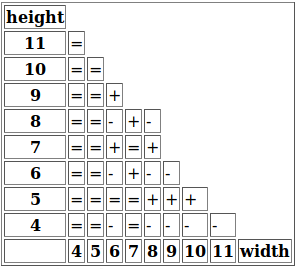
\includegraphics[width=0.7\linewidth]{w-h-viergew}
		\caption{}
		\label{fig:w-h-viergew}
		\footnote{Tromp, John  \glqq John's Connect Four Playground \grqq{} \url{http://tromp.github.io/c4/c4.html} Stand: 01.05.2019}
	\end{figure}
    \newpage
	Zu Abbildung 1:\\
	+ der 1. Spieler gewinnt\\
	- der 2. Spieler gewinnt\\
	= Unentschieden\\
	
	
	
	\subsection{Schwächen}
	Theoretisch sind der KI mit dem Minimax-Algorithmus nur Grenzen gesetzt durch die Rechenleistung bzw. die Tiefe der Simulation.
	
	\subsection{Implementation}
	Die Ki ist in der Klasse AiMiniMax beherbergt. Die dabei wichtigen Methoden sind zum einen die Methoden zum Erzeugen von VierLogik Objekten an denen die Simulationen durchgeführt werden und zum anderen die Umsetzung MiniMax-Algorithmus. Der Aufruf aus VierGame benutzt die Methode aiTurn. In dieser wird jeder Möglichkeit auf ein Feld zu setzen ein Wert durch den MiniMax-Algorithmus zugeordnet und danach wird auf das Feld mit dem höchsten evaluierten Wert gesetzt bzw. auf eines der Felder mit dem höchsten evaluierten Wert. Das Herz der KI ist aber der MiniMax-Algorithmus. Der Aufruf erfolgt damit, das der Zug günstig für den Gegenspieler ist (minimierend für die KI), weil der Zug der KI ja schon für jedes der verfügbaren Felder gemacht wurde, um jedem dieser einen Wert zuzuweisen. Wenn es hier, bei einer der durchprobierten Möglichkeiten für den Gegenspieler zu setzen,  zu einem Sieg des Gegenspielers kommt, wird ein negativer Wert zugewiesen, der depth entspricht und zurückgegeben. Dies sorgt dafür, dass eine spätere Niederlage besser Bewertet wird als frühe. Bei einem Unentschieden ist der Entsprechende Wert 0. Wenn nichts davon eingetreten ist, wird der entsprechende Zug in history gespeichert und der Algorithmus beginnt den nächsten Zug des Spielers zu bewerten. Hier gilt das umgekehrte, da es den Spieler Maximiert. Ein früher Sieg bekommt eine sehr positive Bewertung und im nächsten Aufruf ist es wieder minimierend. Wenn die maximale Suchtiefe erreicht ist wird 0 zurückgegeben und diese Reihenfolge an Zügen wird wie ein Unentschieden behandelt.
	
	\subsection{Effizienzbetrachtung}
	Um mehr Züge zu simulieren ist erheblich mehr Rechenleistung erforderlich. Die Komplexität steigt nahezu exponentiell, aber je weiter das Spiel fortgeschritten ist und je weniger Möglichkeiten es gibt, desto schneller wird der Algorithmus. Ich habe Simulationen durchgeführt mit verschiedenen Feldgrößen und habe den ersten Zug von der KI berechnen lassen, dabei habe ich die Zeit gemessen und damit passende Tiefen gewählt, um die Zeit bei weniger als 10 Sekunden zu halten. Hätte ich die vordefinierten Pfade genommen, wäre deutlich an Rechenzeit gespart worden, jedoch bräuchte man zum Erstellen dieser sehr lange bzw. würde es den Rahmen dieser Facharbeit sprengen. Auch wäre es möglich anstatt der VierLogik Klasse auch einfach nur kopierte Arrays zu verwenden, aber dabei ist es schwer darauf zu achten, dass keines dieser Arrays verändert wird.\\
	Aber nun zur Effizienz bei verschiedenen Feldgrößen. Da die Höhe nicht so ausschlaggebend ist wird hier nur betrachtet wie sich die Ausführungszeit verändert, wenn die Suchtiefe und die Feldbreite variiert werden. Die KI versucht in jedem Fall den ersten Zug eines Spieles zu berechnen.\\
	Im folgenden sind die Graphen der Ausführungszeit im Bezug auf die Suchtiefe dargestellt. Von oben nach unten mit den Feldbreiten 9,7,5. es fällt deutlich auf, dass bis zu einer Suchtiefe von 5 kaum Unterschiede auftreten und von da an die Unterschiede pro weiterer Suchtiefe immer größer werden und exponentiell steigen. Der Wert für die Feldbreite 9 und Suchtiefe 9 fehlt, da ich die Messung nach 2 Stunden abgebrochen habe. Die Tests wurden durchgeführt mit der Klasse Testting.
	
		\centering
		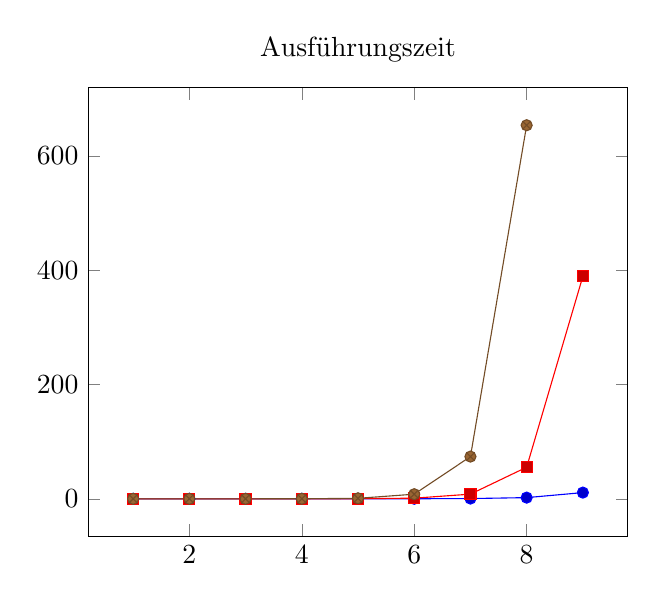
\begin{tikzpicture}
		\begin{axis}[title={Ausführungszeit}]
		\addplot coordinates{%5
			(1,0.002)
			(2,0.001)
			(3,0.007)
			(4,0.027)
			(5,0.022)
			(6,0.122)
			(7,0.451)
			(8,2.104)
			(9,10.888)
		};
		\addplot coordinates{%7
			(1,0.0)
			(2,0.001)
			(3,0.003)
			(4,0.022)
			(5,0.164)
			(6,1.151)
			(7,8.182)
			(8,55.315)
			(9,389.38)
		};
		\addplot coordinates{%9
			(1,0.001)
			(2,0.001)
			(3,0.011)
			(4,0.099)
			(5,0.904)
			(6,8.096)
			(7,73.896)
			(8,653.781)
		};
		\end{axis}
		\end{tikzpicture}
	
	\section{Künstliche Intelligenz}
	\textit{Definition}
	\subsection{Aktueller Stand}
	\textit{tensorflow,machine learning}
	\subsection{Ausblick}
	\textit{Filme usw. (Wargames,Terminator,2001,I Robot)}
	
\end{document}

